\chapitre{Sous le joug d’Ilsa la louve, du 25 au 26 juillet 2033}{En 2002,}{ le docteur Jawad Kebbaj, 30 ans, diplômé de la Faculté de Médecine et de Pharmacie de Rabat, prenait enfin conscience, après quatre années de tergiversations bureaucratiques à Montréal, Québec et Ottawa, que jamais il ne pourrait pratiquer l’art d’Esculape au pays de la castonguette. Le brassage ahurissant de papelards, les retours innombrables à la case de départ, l’arrogance de certaines autorités décisionnelles avaient eu raison du peu de patience dont disposait le Marocain. Comme il aimait démesurément les femmes et qu’il avait des réserves par rapport au Prophète et ses sourates, il choisit de rester et de demander sa citoyenneté canadienne, ce qui lui fut accordé en novembre 2003, malgré les suspicions nées dans la mouvance du 11 septembre 2001. }

Jawad adorait les Québécois, peuple bon enfant qui semblait associer Maroc et bouffe : «Ah, tu es Marocain ? Écoute, j’ai un tajine et je fais souvent du poulet aux olives» ou encore «Ah, tu es Marocain ? Si je te dis comment je prépare mon couscous, vas-tu rire de moi ?» ou encore «Ah, tu es Marocain ? Qu’est-ce que tu penses de l’huile d’olive tunisienne de Sfax ?» Pendant ces quatre années, il avait travaillé dur au souk Sami Fruits du Marché Jean-Talon, il avait fait des heures abrutissantes dans un dépanneur de Villeray et il était devenu chauffeur de taxi non propriétaire dans l’est de Montréal. Mais en 2008, l’amour de sa vie l’avait amené à quitter Montréal pour s’établir dans le quartier Saint-Robert de Rimouski. C’est ainsi que depuis 25 ans, il conduisait son bahut dans la métropole du Bas-Saint-Laurent. Ses clients n’ignoraient pas qu’il avait des réserves par rapport au Prophète et au Coran, mais ils savaient également qu’il ne tolérait absolument pas que l’on manque de respect ni envers l’un, ni envers l’autre. Si en 2033 Jawad Kebbaj ne portait plus le titre de docteur, Il se consolait en voyant ses fils Étienne et Xavier étudier la médecine à l’Université Laval.

- Au lieu d’un docteur Kebbaj, Soubhanallah, il y aura deux docteurs Québage, articulait-il en souriant.

Quand il observe Timothée en train d’attacher sa ceinture sur le siège arrière de son véhicule électrique, il ne peut retenir une remarque.

- Si tu continues à toujours te promener en taxi, il va falloir que je te négocie un forfait, mon jeune homme. Sinon, tu vas te ruiner.

- Bonjour monsieur Kebbaj.

- Ne me dis rien. Laisse-moi deviner. Si tu t’es mis de l’eau de Cologne, c’est que tu t’en vas chez une belle, une belle avec qui tu espères passer de bons moments, tabarnak.

Jawad se voulait Québécois tricoté serré.

- Je vais donc faire diligence, mais sans trop de brusqueries. Je ne veux pas te virer l’estomac en compote. Tu vas avoir besoin de tous tes moyens, mon jeune homme.

\begin{floatingfigure}[l]{40mm}
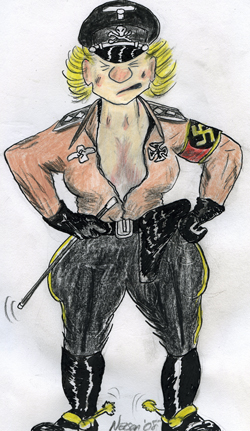
\includegraphics[height=60mm]{corps/chapitre12/img/personnage-marie-odile-ilsa.jpg}
\end{floatingfigure}

C’est avec le sourire de quelqu’un qui boit son thé en sirop ultra sucré, que quinze minutes plus tard, il dépose Timothée devant l’appartement de Marie-Odile. C’est presque en face de l’École Paul-Hubert, l’alma mater de tant d’ânes qui, aujourd’hui, s’en prennent à lui. Avoir perçu ce qui trottait dans la tête de son client, Jawad Kebbaj lui aurait sûrement servi cette perle de la sagesse ancienne, «arbat al bhim ahdha al bhim, mou’almou nhig i’almou chhig», autrement dit «si tu accroches l’âne à côté d’un autre âne, il lui apprendra à braire». Des ânes, des brutes, des éléments de troupeau, des idiots qui ne savent pas ce que c’est que de vivre en cachant de vieux illégaux sur le point d’être débusqués, qui ne savent pas ce que c’est que de marcher avec 1000 kilos de plomb dans sa poche à stress, qui ne savent pas ce que c‘est que jouer du trombone quand on déteste cet émetteur de pouet-pouet qui tue toute possibilité de découvrir l’instrument essentiel à son harmonie de vie, qui ne savent pas ce que c’est que de venir se rapporter à l’heure convenue à une femme flic pour apprendre ce que sa vie sera désormais.

Assis au salon dont l’essentiel du décor lui avait échappé l’autre soir, il remarque qu’aucune bouteille de vin ne décante, qu’il n’y a pas de musique d’ambiance et que Marie-Odile est habillée comme pour aller courir cinq kilomètres dans les feuilles d’un sous-bois. De son fauteuil où elle s’est juchée, les jambes repliées, elle l’observe comme une araignée se pourléchant devant une mouche prisonnière. Pire, comme une mante religieuse face à son petit mâle grotesque. Mais elle perçoit assez vite l’inconfort extrême dont souffre son visiteur et elle choisit d’y mettre fin. Gentillesse ? Compassion ? Magnanimité ? Félinité ?

Elle a beaucoup réfléchi, lui raconte-t-elle. Elle comprend parfaitement sa situation. Il est plus que probable qu’elle aurait agi de la même façon si elle s’était trouvée dans ses chaussettes. Les liens du cœur sont ainsi faits. Dans la vie, on peut être chef de section ou agente de sécurité, on demeure avant tout un fils ou une fille. Le sang parle plus fort que le quotidien d’une carrière. Sauf que le malheur a joué contre lui et l’a placé dans une situation intenable. Des méchants lui en veulent et ils semblent tenir un filon pour le bouffer tout cru. La vie est bien cruelle. Une jungle où les lianes se louent à la minute. Ceci étant dit, il faut se rappeler que tous les égouts mènent à la mer. Il suffit d’avoir un plan et de le suivre méticuleusement. Justement, voyez-vous, elle en a un, de plan. Un plan en quatre points avec, au terme, l’océan ensoleillé et ses effluves.

- Euh ?

Elle lui explique avoir flairé quelques maillons faibles dans l’écheveau de calamités qui caractérise l’ordinaire du pauvre garçon depuis quelque temps, le pire étant le bon docteur Gagnon lui-même. Sa faiblesse ? Il est convaincu de la tendre imbécillité du fils Tardif. Il croit le tenir à sa merci en raison des liens émotifs particuliers à la situation. C’est effectivement une belle faille et c’est par là qu’elle, l’agente de sécurité Marie-Odile Tremblay, matricule 6758AAZ-BSL-01, se glissera et réussira à lui arracher toutes ses dents. À froid.

- J’suis pas sûr de te suivre …

Se basant sur la réputation du CRG-BSL où tout n’est que carambouille, maquignonnage, imposture, crossage et vol, le médecin est convaincu que Timothée trouvera une façon de lui fournir les produits pharmaceutiques dont il a besoin. Il en a demandé cent pour être certain d’en avoir dix. Il lui suffit de savoir doser la pression, de savoir bien étirer l’élastique, de ne rien précipiter, de continuer à ne pas laisser de traces; le brave employé lui ramènera ses médicaments, petit à petit. Mais s’il se fait pincer, le brave employé ? S’il parle ? N’est-ce pas dangereux pour le docteur qui, de par la loi, est tenu de dénoncer des vieillards illégaux quand il en rencontre, ce qu’il n’a pas fait avec les parents de Timothée ? Il peut donc être accusé de complicité, n’est-ce pas ? Pas vraiment. En réalité, si cela se produisait, il plaiderait la compassion. Il dirait qu’entre ses obligations légales auprès du ministère des Affaires gérontologiques et son serment d’Hippocrate le forçant à porter secours à ses frères humains quels qu’ils soient, où qu’ils soient, sans considération lucratives, il aura opté pour la seconde partie de l’équation. Et il n’en dira pas plus sous prétexte de secret professionnel. Tant et si bien qu’il s’en tirera comme bien d’autres l’ont fait avant lui.

- J’ai vérifié et j’ai constaté que depuis l’entrée en vigueur de la loi Turcotte, le gouvernement n’a jamais poursuivi les médecins réputés avoir soigné professionnellement et gratuitement, soi-disant par compassion, des personnes louches en ce qui a trait à l’état civil. Personne ne veut se retrouver en Cour suprême.

- Mais Gagnon exige de se faire payer …

- As-tu une preuve ? Non ? Ce sera ta parole de petit fonctionnaire subalterne du MAG contre celle d’un professionnel influent qui en mène large dans certains cercles rimouskois. Tu te feras planter, ensuite, il te traînera devant les tribunaux pour diffamation. En même temps, tes parents se feront ramasser par les agents du BAG.

Marie-Odile répugnait à utiliser le mot «flic».

- Et ça, tu ne le veux pas. Il faut donc éviter que la situation en vienne là. Mais tu dois bouger vite. À la vitesse où les choses évoluent, c’est certain que tu frappes ton mur de briques d’ici vendredi. Trop de méchants t’ont présentement dans leur collimateur.

- Euh ?

Elle s’est levée et arpente énergiquement son salon.

- Écoute attentivement. La première partie de mon plan consiste à trouver une preuve que Gagnon demande un paiement illicite en retour de ses services. Tu vas donc aller le rencontrer, demain au plus tard, pour négocier un délai d’une semaine. Tu lui diras avoir une combine sûre pour te procurer ce qu’il veut, par exemple une complicité essentielle que tu es en train de développer, mais que tu as besoin d’un peu plus de temps. Soit qu’il accepte, ce qu’il fera si je l’ai bien décodé, soit qu’il refuse, ce qui revient au même. Pourquoi ? Parce que, tout à l‘heure, je vais remplacer le bouton du haut de ta chemise d’uniforme - ça tombe bien que tu ne te sois pas changé avant de venir ici – je vais te le remplacer par le mien qui, comme tu le sais, cache une microcam. Comme ça, tu pourras numériser toute la séquence. À part la couleur, nos chemises d’uniforme sont semblables. Elles sont fabriquées au même endroit et ont les mêmes boutons. Gagnon qui est certain que tu es le pire des caves ne pensera jamais que tu es en train de tout filmer.

- Oui, mais s’il a un petit bidule comme le tien pour brouiller les ondes ?

- Ça m’étonnerait ! Y a personne qui a ça à part les forces de l’ordre.

- Oui, mais ça sera un enregistrement illégal …

- Un enregistrement illégal qui ne pourra être utilisé en cour ? C’est pas pour la cour qu’on fait ça, c’est pour Internet. Il faut que Gagnon sache qu’à tout moment, on peut mettre ça en ligne. C’est une épée de Damoclès sur sa tête, quoi. C’est ce qui va nous permettre de passer à la deuxième partie du plan.

Dieu du ciel que cette femme sait organiser les choses, prendre des décisions et imposer son point de vue !

- Eh ! Oh ! M’écoutes-tu ? fait-elle en se tapant les mains. Allô la Lune ! Tu me suis ?

Elle enchaîne sur le stade suivant, lequel, estime-t-elle, est «un peu plus compliqué». Il repose sur la complicité d’une troisième personne, une personne fiable hors de tout doute, une personne qui, si jamais c’en arrivait là, ce qui serait très étonnant, témoignerait avoir reçu d’urgence, mercredi dernier, des soins confidentiels du bon docteur Étienne Gagnon moyennant juste rétribution.

- Idéalement demain soir, après-demain au plus tard, j’irai cueillir formellement son témoignage, C’est essentiel pour passer à la partie 3 du plan. As-tu quelqu’un pour agir comme troisième personne ?

- Les deux amis sur qui je pourrais compter travaillent au Centre.

- T’as sûrement quelqu’un d’autre?

Il secoue la tête négativement.

- C’est pas une réponse ! Va falloir que tu trouves. Cette personne est LA clé. La fin temporaire de tes ennuis. Du temps que tu gagnes pour mieux t’organiser.

Timothée est découragé. Tout cet échafaudage lui semble tellement tiré d’un mauvais roman policier.

- T’as vingt-quatre heures pour trouver. Après, t’es cuit. Well done ! All dressed !

Surtout que s’il y arrive, elle pourra passer à la troisième étape et faire d’une pierre deux coups. Primo, elle se pointera chez le docteur à qui elle demandera de corroborer le témoignage de la troisième personne. S’il refuse, elle le menacera avec l’enregistrement de la microcam. Secundo, elle se fera un plaisir de le regarder directement dans les yeux pour lui dire d’oublier ses produits pharmaceutiques. S’il les veut absolument, ses foutus produits, il n’aura qu’à venir les voler lui-même en déjouant tous les systèmes de sécurité ou il n’aura qu’à recruter de vrais malfaiteurs pour le faire, le Centre en compte quelques-uns. S’il râle, elle le menacera, encore là, avec l’enregistrement de la microcam. S’il devient violent ? Elle s’amusera. Elle rappelle, non sans délectation, s’être adonnée aux arts martiaux pendant sept ans. Bien sûr, elle était plus mince, mieux musclée, plus souple et, surtout, plus jeune. Mais il lui reste, disons, quelques habiletés pouvant contribuer efficacement à pacifier un toubib devenu désagréable et désorganisé.

Puis ce sera la partie 4, la plus simple du plan de Marie-Odile.

- C’est là où tu me déclares formellement que depuis ton arrivée sur la rue Crouet, ton méchant voisin d’en face n’a jamais cessé de t’enquiquiner et qu’il te déteste parce que ta maison lui bloque la vue. Je présenterai cette histoire comme une chicane entre voisins.

Timothée revoit Richard, être sournois et désagréable s’il en est, en train d’arroser sa pelouse d’un œil et de l’écornifler de l’autre.

- Quand tout cela sera terminé, je téléverserai la synthèse de cette information dans un rapport à l’attention de la direction générale. On y apprendra que mercredi dernier, tu as dépanné une personne de ton entourage, une personne qui, pour des raisons personnelles et confidentielles, préfère utiliser le secteur privé du réseau de la santé en allant chercher le docteur Gagnon, lequel a été dûment payé pour ses services, ce qui est parfaitement légal. Puis j’ajouterai des explications quant à ton idiot de voisin. Et je signerai. Ça devrait geler Dauphin et Michaud «pour quelque temps».

- Euh … et Richard, de l’autre côté de la rue ?

- Lui ? S’il veut déconner, je vais lui faire la peur de sa vie, il va nous foutre la paix !

Mais attention, insiste-t-elle. La notion de «pour quelque temps» est ici très importante. Le voisin aura beau être rationalisé, les hommes de Flipper neutralisés, il se sera dit des choses. Il y aura possiblement des traces. Des rancœurs. Et il n’y a jamais de fumée sans feu. Pourquoi Dauphin, pour le jouissif plaisir de se venger, n’enregistrerait-il pas une dénonciation anonyme auprès du Bureau des affaires gérontologiques, le BAG ? Ou pourquoi Richard ne le ferait-il pas, ou le docteur Gagnon ou un autre qui aurait pu voir passer l’information ? C’est leur devoir de citoyen de le faire, non ? Bref, il est certain que la maison de la rue Crouet va, un jour, peut-être dans un mois, peut-être dans un an, recevoir la visite des flics du BAG.

- Seigneur que c’est angoissant tout ça !

Marie-Odile, en route vers la cuisine, hausse les épaules. Timothée l’entend ouvrir le réfrigérateur, puis bardasser autour.

- Évidemment, fait-elle la tête dans une armoire à verres, ce sera donnant donnant.

Ça y est, se dit-il, voici la facture et elle ne peut être qu’étourdissante ! Mais prudemment, il évite de répondre et se place en mode attente, ce qui ne dure pas une éternité. Cabaret en main, Marie-Odile revient avec un muscadet de bonne mine, deux coupes et des biscottes. Seigneur !

- Ça t’intrigue pas plus que ça de savoir ce que j’entends par «donnant donnant» ?

- Euh …

Elle sourit largement et s’active avec le tire-bouchon.

- C’est l’autre côté de la feuille où j’ai écrit le plan que je viens de t’expliquer !

Timothée se lève pour l’aider dans sa tâche sommelière, mais il est trop tard, pop!, la bouteille a été ouverte.

- Ça va aller, tu peux te rasseoir.

Pendant qu’elle emplit les verres, elle lui rappelle lui avoir parlé, vendredi, de ses parents, deux désespérés à la veille de devoir être internés au Centre. Un bien grand malheur ! Si ce n’est pas la diète au Nutrisuz, alias le manger mou, qui les emportera en moins d’un an, ce seront les mauvais traitements et le manque d’hygiène. Il faut donc trouver une meilleure solution et, justement, elle a songé à quelque chose de potentiellement pas trop désastreux. Elle a d’abord imaginé les faire passer sur l’île d’Anticosti, mais son père n’a pas la santé suffisante; il y serait très malheureux. Elle a ensuite réfléchi sur une sorte de mise en commun. Elle, toute seule, ne peut arriver à entretenir ses vieux. Elle ne dispose ni du temps ni des moyens nécessaires. À plus forte raison que s’ils deviennent illégaux, ils perdront leurs revenus de pensions. Lui, Timothée, c’est exactement la même chose; son état actuel de détresse en est une belle preuve. La solution serait donc de tout vendre, la maison de ses parents à elle et celle des Tardif, rue Crouet, puis d’acheter «plus grand ailleurs», dans un rayon de 50 kilomètres de leur travail, en priorisant les propriétés relativement … isolées. Dans cette hypothèse, on aménagerait des espaces privés pour respecter l’intimité des gens. Mais il y a des risques. Imaginons que les deux couples ne s’entendent pas ou qu’une telle adversité leur arrive à elle et à lui.

- Pourtant, on n’a pas le choix.

La vitesse et la maestria avec lesquelles l’employée de la Sécu est en train de l’embobiner dans un cocon à sécurité maximale font frémir Timothée.

- Donc, conclut-elle, on va se mettre à l’ouvrage.

La série noire et sa liste de catastrophes continuent. Ce qui tend à démontrer qu’au moment où on croit toucher le fond, il est toujours possible d’aller plus creux. Le rationnel est pourtant simple : toute situation en dégénérescence a une vitesse de bordélisation qui équivaut à la somme des efforts consentis pour l’enrayer, multipliée par le nombre de jours écoulés depuis le début. On jurerait entendre Robespierre.

- Tu m’écoutes ?

Les yeux qu’il lui adresse sont ceux du caribou qui scrute un chasseur d’allure joviale en train de lui faire signe de ne pas bouger parce que tout va bien se passer.

- On va mettre des locataires dans ta maison, ce qui va rapporter des sous. De mon côté, je vais en faire autant avec mon condo. En même temps, je vais vendre le bungalow familial et, une fois l’hypothèque, les prêts et les frais remboursés, il devrait me rester assez d’argent pour payer «nos» coûts de réno dans la nouvelle demeure où on va aménager quatre logements : un pour toi, un pour moi, un pour mes parents et un autre pour les tiens. Chaque mois, je vais verser mille dollars dans ton compte pour que tu t’assures que personne ne manque de quoi que ce soit. En plus, je vais t’aider avec les courses. Ça va nous permettre de nous voir de temps en temps, ajoute la femme flic en clignant de l’œil. Qu’est-ce que t’en dis ?

Une fois ces lourdes responsabilités distribuées à son entière satisfaction, elle a vidé son verre d’un trait et s’est levée.

- Pis, mon plan ?

- Euh …

En moins de temps qu’il en faut à un homard pour accéder à la boette au fond de la trappe, Timothée se retrouve dans les draps de la maîtresse femme qui lui fait rapidement exulter l’exaltable. Même qu’elle le complimente sur sa prestation, une nette amélioration sur les autres fois. Si si ! Mais, il ne faut surtout pas en rester là, n’est-ce pas ? La vie est si courte. Allez, mon beau Timo ! À l’attaque ! Oh hisse ! Du nerf ! Sursum corda ! En soupirant, le pauvre diable pense à ce que doit être le quotidien du godemichet dont il aperçoit la base dans le tiroir mal fermé de la table de chevet.

- Ouille ouille ouille, mon jeune homme ! Tu as toute la luxure de l’enfer des chrétiens étampée au visage.

Timothée que Marie-Odile vient de renvoyer chez lui en taxi, non sans lui avoir rappelé les consignes du lendemain en lui remplaçant le premier bouton de sa chemise d’uniforme, regarde le chauffeur.

- Vous travaillez beaucoup, monsieur Kebbaj.

- Y a ma moukère qui dit que la vie coûte cher, tabarnak.

Quelques courtes heures plus tard, Timothée poireaute à côté de Dart Vader dans le bureau de Philippe Dauphin. Plus tôt, en arrivant à son officine du 5e Nord, il avait pris note de cette convocation d’urgence lui ordonnant de se présenter à la direction des communications en compagnie du bénéficiaire Robert Gagnon. Mais depuis cinq minutes qu’ils font face tous les deux au superbe meuble en acajou qu’utilise le Flipper pour bien camper son pouvoir, personne ne s’est encore occupé d’eux. On leur a crié d’entrer et on les a ignorés. Quand Dauphin n’est pas au téléphone, il donne des ordres à ses sbires qui vont et viennent ici et là, incluant dans la cuisinette adjacente au grand bureau. À ce que comprend le CS-1, le branle-bas semble attribuable à la réunion du conseil d’administration prévue pour le lendemain matin.

- Peux-tu vérifier qu’en fin de journée, aujourd’hui, tous les véhicules du Centre soient bien alignés dans le stationnement ? s’informe le Flipper à une adjointe à la mine peu réjouie.

- Pas de problèmes, Philippe.

- As-tu demandé à quelqu’un de faire le rappel habituel ?

- J’ai fait ça moi-même, hier soir. Ça va te coûter des heures sup, boss !

- À quelle heure les traiteurs vont venir porter leurs plats de bouffe ? crie-t-il encore à Claude Sey occupé dans le coin-repas.

- Je leur ai dit de passer entre 21 h 30 et 22 h, entend-on. C’est l’heure où le concierge vient faire le ménage; les portes sont débarrées.

Clouc ! Les yeux de Dart Vader viennent soudainement de s’illuminer.

Après un dernier téléphone et une ultime manipulation sur son terminal, Dauphin, drapé dans un costar de riche et cravaté de rouge, dévisage au travers de ses foutus binocles de soi-disant intello, ses deux «convoqués» avec tout le mépris dont il est capable et, c’est connu, son registre est très développé. Sans les saluer, il les apostrophe d’entrée de jeu. Il se dit furieux, humilié, il veut des explications, des excuses. Depuis quand un employé subalterne peut-il court-circuiter la décision d’un directeur ? Si Gagnon était en «cellule de réflexion», c’est qu’il y avait de bonnes raisons, que les intérêts supérieurs du CRG-BSL étaient en cause. Si n’importe qui commence à faire n’importe quoi dans cet établissement, rien n’ira plus. En un mot, cette histoire ne restera pas là.

- Ça vient de te coûter ta job, le cave ! Attends que j’en parle à Carl !

Timothée regarde en silence cette onzième plaie d’Égypte lui débarquer sur le bide et lui coller à la peau.

L’adjointe aux «heures sup» pointe son joli nez, côté jardin.

- La Sécu est arrivée.

- Fais-les rentrer.

Le temps de passer en revue tous les chapitres de la petite apocalypse qui l’habite depuis quelques jours, Timothée voit apparaître, côté cour, Marie-Odile et Tropecolo le Chinois.

- Vous allez me ramener ce vieux malfaiteur dans le trou d’où vous l’avez laissé filer hier, avez-vous compris ?

Tropecolo se gratte le crâne aux poils ras.

- Pour quel motif ?

- Ordre de la direction générale.

- Il est où cet ordre ? Justement, je ne l’ai pas trouvé hier.

- Laisse faire la paperasse ! Sortez-moi ça de mon bureau !

- On peut pas enfermer les gens comme ça. Ça prend un ordre signé par quelqu’un d’autorisé.

- Écoute, le Chinois, fais pas le «smatte» ! Je te dis de descendre ce vieux sac à merde et tu vas le faire. C’tu clair ?

- Moi, le Flipper, je te dis «pas d’ordre signé, pas d’emprisonnement». Rappelle-nous quand tu en auras un.

\begin{floatingfigure}[l]{40mm}
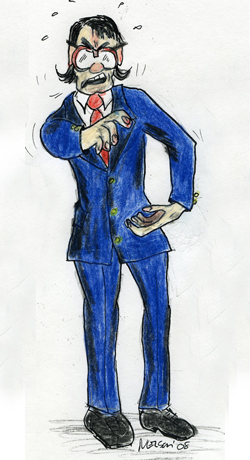
\includegraphics[height=60mm]{corps/chapitre12/img/personnage-dauphin.jpg}
\end{floatingfigure}

Il fait signe à sa collègue et tous deux déguerpissent malgré la rage évidente du satrape de la haute direction. Ce que Timothée croit décoder, c’est que les jours du Chinois sont non seulement comptés, mais qu’ils lui seront très douloureux à vivre. Idem pour Marie-Odile. Il aurait envie de cracher quelques bons sarcasmes, mais ce n’est pas dans sa nature et il se contente de donner un léger coup de coude à Dart Vader.

- Nous autres, Flipper, on va en faire autant. Tu sais où nous joindre !

- J’vous ai pas dit de partir ! Et mon nom c’est Dauphin, pas Flipper !

Dart Vader s’approche du bureaucrate et referme sa canule.

- Écoute-moi b’en, mon astie d’face de trou de cul, tu m’as fait passer six jours dans une cage du sous-sol, b’en j’vas t’le faire regretter pour le restant de tes jours ! Compte sur moi ! Tu vas apprendre qu’à mon âge, on n’a pas six jours à perdre comme ça !

Et, bras d’honneur à l’appui, le bonhomme fait volte-face et sort du bureau, son CS-1 lui emboîtant le pas.

Se pourrait-il que la vie terrestre, celle des humains, soit un divertissement adulte que s’offrent des forces inconnues, une sorte de mégajeu vidéo avec des cartes gagnantes, par exemple celle du IIIe Reich qui donne droit à quinze millions de morts ou celle de l’Encomienda à sept millions, et des cartes perdantes, par exemple celle de la guerre anglo-argentine qui ne donne même pas mille morts ou, pire, celle de l’invasion de la Grenade où il y a moins de cent décès ? Se pourrait-il que le Grand Ordonnancier qui a programmé ce jeu soit devenu cinglé ou soit couché en permanence avec une pipe d’opium collée au bec ? En attendant de résoudre cette énigme, Timothée décide de profiter de son passage au rez-de-chaussée pour se rendre aux services techniques. On ne sait jamais, se dit-il sans trop d’espoir.

Mais, à bien y penser, pourquoi lui remettrait-on un DPP tout neuf quand tellement de possibilités néfastes peuvent les en empêcher ? On a l’embarras du choix : le département sera fermé, le modèle qui lui est destiné sera en rupture de stock, une opération d’inventaire sera en cours, le préposé ne trouvera pas les clés de l’armoire, un météorite sera tombé sur le local, n’importe quoi.

Effectivement, rendu sur place, il constate que si ses appréhensions étaient fondées, il n’a pu en imaginer la raison.

- Écoute, Motté, je peux pas t’en donner un neuf, lui explique l’obèse derrière le guichet de service. C’est marqué, ici, que tu fais l’objet d’une enquête.

Il peut arriver qu’on ait la certitude qu’un disjoncteur cérébral va céder et que 43 ans de colère seront déversés sur un misérable fonctionnaire qui aura commis l’erreur d’ânonner l’imbécillité normative ultime, celle qui aura fait déborder le vase. Si c’est ce que Timothée ressent, rien ne paraît, sinon un léger agacement.

- Enquête mon œil, c’est une connerie du Flipper.

- R’garde, c’est inscrit ici. J’y peux rien. Si fais l’objet d’une enquête, on peut rien te donner; c’est le règlement. Va te «clairer» de ça et reviens nous voir !

Et shlack!, le gaillard referme le guichet, confirmant le très frustré chef de section dans son rôle de perdant venu au monde pour une tranche de pain moisi, de musicien hypersensible à qui on n’a remis qu’un méchant trombone, de Timothée de Saint-Anaclet que des parents ont confondu avec Timothée de Milet, de cave sans importance que des lèche-culs font parader dans leur bureau à côté d’un petit vieux à canule, de baiseur néophyte à qui une ancienne karatéka tetonnée accorde une note de passage, de mangeur en série de pizza qui se fait zigner par un chien laid à pleurer. Hurler ? Frapper ? Mettre le feu ? Tout faire sauter ? Ou, comme il a toujours fait, laisser «border» ?

Laisser «border» comme cette fois, c’était l’hiver, où des condisciples du Paul-Hubert, en mal de sensations fortes, l’avaient encerclé en le moquant du mieux que leur piètre vocabulaire le permettait. Redoux aidant, ils étaient plus nombreux qu’à l’accoutumée à flâner sur le trottoir entre le parc et l’école. Attaquant en meute, ils lui avaient arraché son manteau, sa tuque et ses gants. Puis, ils s’en étaient pris à son sac d’écolier, éparpillant son contenu à hue et à dia. Enfin, ils lui avaient glissé de la neige sale dans le dos, sous sa chemise.

Une kyrielle d’enchaînements injustes avait alors déferlé. N’ayant plus en sa possession le matériel requis pour suivre en classe, essentiellement des manuels et des cahiers d’exercices, tous déchiquetés sadiquement, il avait été puni par le professeur de français et expulsé par sa collègue en mathématiques. De plus, n’ayant pu leur remettre les travaux hebdomadaires entendus pour cause de dissémination aux quatre vents, incluant ceux destinés aux profs d’anglais et d’histoire géographie, il avait reçu quelques zéros et avait été consigné à la retenue du samedi, ce qui impliquait d’être reconduit à l’école par son père, le transport scolaire n’étant pas accessible les fins de semaine. Pire, le fait de devoir retourner à la maison sans vêtements chauds lui avait fait prendre froid et il avait été malade pendant une bonne semaine sans que sa mère lui permette de garder le lit comme le réclamait son état. En fait, c’est la Maririou qui s‘était alors avérée la plus terrible conséquence; sa colère avait été à la hauteur du crime. Comment se pouvait-il qu’à son âge il «perde ses affaires comme un bébé de maternelle» ? Il n’était qu’un «grand niaiseux», un «étourdi», un «immature», un «nono», une «honte pour ses parents». Comme punition, il avait été privé de télé et de dessert pendant presque un mois; Romain avait dû intervenir pour qu’elle le gracie. Eut-il dit la vérité au lieu de baragouiner de vagues «j’sais pas moi», la sentence maternelle aurait été pire encore. «T’es pas capable de te défendre, espèce d’innocent ?»

On avait bien ri au Paul-Hubert.

Timothée revoit ce barbu resplendissant de santé l’aborder, il y a deux ans, dans un centre commercial.

- Timothée Tardif ?

- Euh … oui ?

- Tu étais au Paul-Hubert en 2005 ?

- Euh … oui ?

- Je sais pas si tu me replaces ? Gilles-André Voyer, moi aussi j’étais au Paul-Hubert. Le jour où tu t’es fait attaquer, que tu t’es fait enlever ton linge et ton sac, je faisais partie de la gang. Sur le coup, j’ai bien ri. Mais le lendemain, j’ai commencé à avoir des remords. Cent fois, j’ai voulu aller te trouver pour m’excuser. Je l’ai jamais fait et je l’ai toujours regretté. Aujourd’hui, je t’ai vu arriver, je me suis dit, c’est Tardif, c’est lui. Faut que j’y aille. Fait que là, je t’offre mes excuses. J’ai agi en «sans cervelle».

Et il était reparti sans saluer, s’étant contenté de se faire du bien.

Pourquoi les autres ne l’ont-ils pas fait ? Il y en a qui exercent présentement des emplois importants où ils sont sûrement appréciés, des salauds que la vie a bien gâtés, eux. Ils ont des familles, une conjointe et des enfants qui les aiment. Probablement. Ce sont des leaders, des «influenceurs», des «battants», des «gagnants», des actifs socio-économiques, des gens utiles. Certains font même parler d’eux dans les médias. Et il y en a deux, pourtant pas les moins pires, qui sont des flics gradés du Bureau des affaires gérontologiques (BAG). Pourtant, ils se sont déjà attaqués à lui comme des hyènes sans qu’ils n’en subissent les effets pervers. Ils ont un voilier, un chalet à Métis, ils voyagent en Europe, ils sont membres du club de golf du Bic, ils ont de gros placements. Pourquoi est-ce ainsi ? Pourquoi n’y a-t-il jamais de conséquences à s’acharner sur les Timothée Tardif de la Terre ? Est-ce sa raison d’être, à lui le fils de la Maririou ? Permettre à du futur bon monde, en tout cas, à de futures «forces vives du milieu», de connaître au moins une fois dans leur vie, ce que c’est que d’être brutal, injuste et vraiment enfoiré ? Et, tant qu’à y être, pourquoi sont-ce ces Flipper Dauphin, ces Carl Michaud, ces Étienne Gagnon, ces fils de pute qui ne s’émeuvent que pour leurs petits intérêts personnels, qui finissent par faire la loi partout, qui gravissent les échelons de la société, qui aboutissent maire, député, ministre, président, qui mettent les vieux en cage sous les applaudissements de tout un chacun ? Les gentils, les doux, les honnêtes, les «qui aiment les vieux» eux, ils ont des lunettes épaisses, des bedons, un début de calvitie. Ils n’ont pas de Saguewanish, pas de boucle d’oreille et sont en train de se faire embrigader dans une relation étouffante par une femme flic, par une émule de Ilsa la louve des SS.

- Pourquoi, câlisse !

Comme un ahuri se parlant tout seul, il prend l’ascenseur sans remarquer Vlado Marcovski, le furtif directeur de l’informatique qui en sort et qui semble ravi de ne pas avoir eu à le saluer. L’eut-il vu qu’il l’aurait sans doute ajouté à sa liste des «fils de pute». À plus forte raison que depuis ce matin, plus rien ne va du côté systèmes; c’est la panne générale. Michaud doit être en train de constituer un peloton d’exécution et Dauphin, en train d’équiper une salle de torture quelque part au sous-sol.

Arrivé au 5e, Timothée consent sans trop réfléchir à une demande de Martel qui veut passer la nuit dans la «petite chambre» avec sa conjointe.

- Ronnie Ross m’a dit de voir ça avec vous, Chef.

Laissant le vieillard perplexe, il file directement chez Robespierre, sans un regard pour Jean Saint-Gelais qui veut le féliciter pour son attitude vis-à-vis Dart Vader, sans ralentir devant une nouvelle supplique de Mme Loubert concernant, cette fois, la qualité des sacs pour colostomie qu’on lui a remis la semaine dernière.

- C’est de la cochonnerie, ils coulent, vos sacs. Je suis obligée de laver sans cesse mes vieux de l’autre jour.

- J’ai pas l’temps, madame Loubert, voyez ça avec Ronnie Ross.

Occupé à pousser ses 300 pompes de la matinée, Robespierre ne dit pas un mot quand son ami entre sans frapper. Discrètement, Mme Bellow qui était occupée à compléter des fiches, quitte sans faire voir de rien.

- Je tchôque !

L’homme fort se relève et s’enroule une serviette autour du coup. Dans les petits haut-parleurs, Léo ferré chante «L’âge d’or» :

    Nous aurons la mer
    À deux pas de l’étoile
    Les jours de grand vent
    Nous aurons l’hiver
    Avec une cigale
    Dans ses cheveux blancs
    Nous aurons l’amour
    Dedans tous nos problèmes
    Et tous les discours
    Finiront par Je t’aime
    Vienne vienne alors
    Vienne l’âge d’or…

- Quelle naïveté, ça date de 70 ans, fait-il en stoppant son lecteur multimédia.

- Tu pues ! lui répond le fils Tardif qui tente de se travailler une contenance. Pauvre madame Bellow !

- Normal, je sens le neg’!

- Ouin !

- Je t’écoute.

Sans ratures ni hyperboles, il raconte au docteur Robespierre ce que, selon Marie-Odile Tremblay, il doit faire tout de suite s’il veut être encore vivant et, possiblement bien portant, dans un jour ou deux. Primo, numériser subrepticement des propos compromettants chez Étienne Gagnon, secundo, trouver une personne voulant se prêter gratuitement à un parjure. Rien que cela !

- Il est génial son plan !

Timothée le regarde, dérouté.

- Génial ! Et j’ai justement la personne qu’il te faut pour le témoignage. Et tu sais qui, d’ailleurs !

- Euh ?

- Pense ! C’est une idéaliste qui est allée organiser un dispensaire en Haïti, une infirmière qui déteste les gros requins de la médecine, une femme que le mot Nutrisuz indispose au plus haut point …

- Ta copine Béatrice qui m’a donné la lettre de Marceline ?

- Ouaip ! Comme je la connais, ça devrait marcher. Je vais t’arranger le coup après l’ouvrage. Si elle veut pas, ce qui m’étonnerait, je vais essayer de trouver quelqu’un; fais-toi z’en pas. Quant à l’autre élément de ton histoire de fous, t’as pas besoin de moi. Tu vas voir ce salopard, tu lui fais ta passe-passe et, couic, il est cuit. La seule difficulté est d’activer la caméra sans qu’il s’en aperçoive. Fais-la démarrer avant d’entrer dans son bureau.

Timothée se retient pour ne pas pleurer et esquisse un mouvement pour disparaître.

- Attends, merde !

Robespierre tape sa boucle d’oreille, demande la direction médicale et, du même ton que s’il avait communiqué avec l’assistance annuaire, s’informe des disponibilités au Centre du docteur Gagnon. On lui répond que le médecin ne passera pas avant après-demain et que, d’ici là, il est possible de le joindre à son cabinet privé.

- Tiens, prends mes clés de char, ça va aller plus vite qu’à pied et ça va te coûter moins cher qu’en taxi.

En moins d’une heure, Timothée réussit ainsi à se rendre à la clinique, à se faire introduire chez le brave docteur entre deux rendez-vous, à se négocier un délai supplémentaire pour le début de ses livraisons – il a tenté une semaine, mais Gagnon ne lui a finalement consenti que quatre jours - et à revenir au Centre où il se présente dans les locaux de la Sécurité.

Sourire aux lèvres comme s’il était l’Agent 007 lui-même, il salue Marie-Odile sans trouver de patère pour jeter son chapeau que, du reste, il n’a pas. Silencieusement, il pointe du doigt son premier bouton et, d’un geste de la tête, laisse entendre que sa pêche aux connards a été fructueuse. Si la femme flic est impressionnée, elle n’en fait rien paraître. Plutôt, elle sort un petit couteau de sa poche et lui fait sauter le bouton en question.

- Oups ! Oh ! As-tu remarqué, il te manque un bouton ?

On échange des sourires complices et le redoutable espion s’approche de la porte.

- Tu vas voir que Gagnon est très clair, il n’y a pas d’équivoque possible, sur les produits qu’il me demande de lui livrer et sur l’outil de chantage qu’il utilise pour me forcer. Pour l’autre partie, la troisième personne, c’est sur rails et je t’en reparle demain !

- Pas ce soir, minaude-t-elle ?

- Demain.

- Mais ce soir, on pourrait … tu sais … Je t’attends vers 20 heures ?

- Euh …

- File ! J’ai du travail. À ce soir.

La bonne nouvelle, Marie-Odile a l’enregistrement. La mauvaise, elle le tient du même coup. Ce qui lui fait penser, en récapitulant sa récente vie d’adulte sexuellement actif, que le prix à payer pour pouvoir tirer honnêtement son coup est très élevé. Les à-côté, les avants et les après de la partouze proprement dite sont considérables. Du temps de son holotar, la branlette de conclusion était infiniment moins lourde à supporter. Or, il paraîtrait que si on est en amour, il n’y a plus rien à endurer, ni avant, ni après, ni à côté. La relation est d’une félicité constante et l’acte sexuel ne vient qu’ajouter à l’agrément. Pour l’instant, il se trouve loin de cette image et rien ne lui indique que ce sera avec Marie-Odile qu’il pourra atteindre cet état de nirvana. Bien au contraire, tout ce qu’il entrevoit avec cette forte femme, ce sont des chausse-trappes, des barreaux de cage, des contrôles serrés, des vérifications incessantes, des miradors entourés de doberman et de rottweillers, des façons de faire auxquelles il a été habitué avec la Maririou, grâce auxquelles il a souffert et il souffre encore, avec lesquelles il ne peut plus vivre.

Sa montre lui indiquant 13 h 55, il hésite entre remonter au 5e faire face au zoo qui l’attend ou descendre au rez-de-chaussée aller voir Shimoune Saint-Pierre qui tient absolument à lui parler et dont la pause repas commence dans cinq minutes. À l’instar de Robespierre, le préposé au manger mou, alias la Grande Folle, est généralement de bon conseil. Aussi bien lui rendre visite. Mais Sébastien Larose, le dernier syndiqué de la fonction publique du Québec, l’interpelle directement de son bureau, un coqueron parfaitement inutile dont la porte est toujours ouverte.

- Aille, mon homme !

Timothée le salue de la main.

- Ça tombe bien que tu passes dans le coin. Je cherche un mot de 13 lettres qui commence par un P, qui finit par un N et p’is que la sixième lettre est un R.

- Euh …

- Ça veut dire : «Action d’améliorer unilatéralement ses conditions de travail dans les hautes sphères de certaines administrations publiques.»

- 13 lettres ?

- Oui.

Timothée compte un instant sur ses doigts.

- PRÉVARICATION !

- Aille mon homme, t’es vraiment capab’ toi ! Merci.

Avant de se faire attraper pour une nouvelle requête, le CS-1 file vers les escaliers et dégringole jusqu’à la cafétéria où il est accueilli par un regrettable «Tiens si c’est pas le beau Momo !»

- Moman que t’as pas d’l’air en forme, toi ! Tu r’sembles à un mort qui a mal ressuscité. As-tu bouffé au moins ? J’ai une glacière dans mon char avec des fruits, du fromage, des viandes froides. Y a même un litre de jus d’ananas. Je m’en allais manger ça en prenant le soleil. Ça te tente de partager ?

- Euh … je ne veux pas t’enlever le pain de la bouche.

- Mon de doux ! J’en ai en masse, s’il y en a pour un, il y en a pour deux, Momo ! De toute façon, j’ai une méchante histoire à te conter. Viens !

Le soleil étant trop violent pour Timothée, Shimoune accepte de surseoir à son rituel de bronzage. Glacière en main, tous deux s’en vont s’asseoir à l’ombre des grands sorbiers près de l’aile sud.

Mais loin de là, à l’extrémité éloignée de l’édifice, un homme a commencé à appliquer le plan qu’il a ourdi depuis le matin. Sur sa chaise de dortoir,Dart Vader, un vieux calepin sur la cuisse, est en train d’écrire au directeur général Carl Michaud, ce que ni Timothée, ni Shimoune ne peuvent savoir, occupés qu’ils sont à bien autre chose.

- T’es cuit Momo ! Les mémères qui nous observent sont déjà parties placoter partout que je m’en vais te sauter dans les buissons.

- Y a p’us rien qui peut m’écœurer, Shimoune. Y a p’us de place !

- Ouh-la-la !

- Je suis devenu un esclave, une larve, une merde. Pire qu’avant. Je suis passé du contrôle de ma mère à celui d’Ilsa, la louve des SS.

Shimoune émet un long sifflement.

- Qui c’est, Ilsa la louve ?

- Un personnage de dominatrice dans un vieux film des années 70.

- Je ne suis pas certain de te suivre. T’es quand même pas en train de me parler de la Tremblay ?

- Oui

Le préposé au manger mou pourrait répondre qu’il l’avait bien prévenu, qu’il ne fallait que s’en prendre à lui-même, que c’était couru. Mais il cache sa pensée. Par tact. De toute façon, ils ont beaucoup mieux à se dire, en tout cas, lui, Shimoune, il a de l’information qui devrait faire son petit effet.

Une fois la glacière ouverte, Le CS-1 réalise que les rations sont peu copieuses, ce qui lui en dit long sur la générosité de son ami. Son ami Shimoune, un marginal comme Robespierre, jovial descendant d’une longue lignée d’Alcide antillais. Marginal comme lui, gras du bide binoclard dont on se moque au Centre. Marginal non pas comme gai-assumé chez les hétéros, noir-fier chez les blancs, ou exclu-timide chez les grégaires, mais comme contrastant par rapport aux autres employés, tout empesés selon les diktats d’un même sale moule.

Dans les deux heures qui suivront, plus Shimoune va avancer dans son récit, plus la relative faim que Timothée ressentait va le quitter. C’est que les faits étalés changeront carrément le cours de la vie du fils Tardif. D’une part, ils lui offriront une raison pour résister aux charmes envahissants d’Ilsa la louve. D’autre part, pour la seconde fois de la journée, un ami lui fera entrevoir de la vraie lumière au bout de son tuyau d’égout.